\documentclass{beamer}
\usepackage{graphicx}
\usepackage{graphics}
\usepackage{fancyhdr}
%\usepackage[OT1]{fontenc}
%\renewcommand*\familydefault{\sfdefault}
\usepackage{amsfonts}
\usepackage{amsmath}
\usepackage{amssymb}
\usepackage{amsthm}
\usepackage{tikz-cd}
\usepackage[most]{tcolorbox}
\usepackage{varwidth}
\usepackage[dvipsnames]{xcolor}
\usepackage{parskip}
\usepackage{fourier-orns}
\usepackage{pgfornament} 
\usepackage{quiver} 
\usepackage{enumerate}
\usepackage{subcaption}
\usepackage{subfig}
\usepackage{subfigure}
\usepackage{animate}
\newcommand{\R}{{\mathbb R}}
\newcommand{\N}{{\mathbb N}}
\newcommand{\Z}{{\mathbb Z}}
\newcommand{\Q}{{\mathbb Q}}
\newcommand{\C}{{\mathbb C}}
\newcommand{\p}{{\mathbb{P}}}
\newcommand{\E}{{\mathbb{E}}}
\newcommand{\la}{\langle}
\newcommand{\ra}{\rangle}
\newcommand{\lt}{\left}
\newcommand{\rt}{\right}
\newcommand{\Cov}{\text{Cov}}
\newcommand{\Var}{\text{Var}}
\newcommand{\wt}{\widetilde}
\newcommand{\eps}{\varepsilon}
\newcommand{\ph}{\varphi}
\newcommand{\Hom}{\text{Hom}}
\newcommand{\im}{\text{Im}}
\newcommand{\mm}[1]{\mathcal{#1}}
\newcommand{\set}[2]{{\left\{ \left.{#1 \vphantom{#2}} ~ \right. : ~ {#2} \vphantom{#1}\right\}}}
\newcommand{\supp}{{\mathrm{supp~}}}
\newcommand{\mathfont}{\mathbf}
\newcommand{\ZZ}{\mathfont Z}
\newcommand{\Zhat}{\widehat{\ZZ}}
\newcommand{\QQ}{\mathfont Q}
\newcommand{\Qbar}{\overline{\QQ}}
\newcommand{\Fbar}{\overline{\FF}}
\newcommand{\ttm}[4]{\begin{bmatrix}
#1 & #2 \\
#3 & #4
\end{bmatrix}}
\newcommand{\fm}{\mathfrak{m}}
\newcommand{\fp}{\mathfrak{p}}
\newcommand{\fq}{\mathfrak{q}}
\newcommand{\qfrak}{\mathfrak{q}}
\newcommand{\into}{\hookrightarrow}
\newcommand{\onto}{\twoheadrightarrow}
%algebra
\DeclareMathOperator{\Id}{Id}
\DeclareMathOperator{\Ker}{ker}
\DeclareMathOperator{\Coker}{coker}
\DeclareMathOperator{\coker} {coker}
\newcommand \tensor[1] {\otimes_{#1}}
\DeclareMathOperator{\Aut}{Aut}
\DeclareMathOperator{\Gal}{Gal}
\DeclareMathOperator{\tr}{tr}
\DeclareMathOperator{\End}{End}
\DeclareMathOperator{\ord}{ord}
\DeclareMathOperator{\val}{val}
\newcommand{\dual}{\vee}
\DeclareMathOperator{\Char}{char}
\DeclareMathOperator{\rank}{rank}
\DeclareMathOperator{\Rep}{Rep}
\DeclareMathOperator{\univ}{univ}
\newcommand{\kbar}{\bar{k}}
\DeclareMathOperator{\Ext}{Ext}
\DeclareMathOperator{\Tor}{Tor}
\DeclareMathOperator{\Res}{Res}
\DeclareMathOperator{\Ind}{Ind}
\newcommand{\Norm}{\mathrm{Norm}}
\newcommand{\Tr}{\mathrm{Tr}}
\DeclareMathOperator{\Sym}{Sym}
\DeclareMathOperator{\der}{der}
\DeclareMathOperator{\tors}{tors}
\DeclareMathOperator{\Fil}{Fil}
\DeclareMathOperator{\gr}{gr}
\DeclareMathOperator{\Gr}{Gr}
\DeclareMathOperator{\Nilp}{Nilp}
\DeclareMathOperator{\Mat}{Mat}
%theorems
\theoremstyle{plain}
\newtheorem{lem}{Lemma}
\newtheorem{thm}[lem]{Theorem}
\newtheorem{prop}[lem]{Proposition}
\newtheorem{cor}[lem]{Corollary}
\newtheorem{conj}[lem]{Conjecture}
\newtheorem{exercise}[lem]{Exercise}
\theoremstyle{definition}
\newtheorem{defn}[lem]{Definition}
\newtheorem{remark}[lem]{Remark}
%caligraphic
\newcommand{\cA}{\mathcal{A}}
\newcommand{\cB}{\mathcal{B}}
\newcommand{\cC}{\mathcal{C}}
\newcommand{\cD}{\mathcal{D}}
\newcommand{\cE}{\mathcal{E}}
\newcommand{\cF}{\mathcal{F}}
\newcommand{\cG}{\mathcal{G}}
\newcommand{\cH}{\mathcal{H}}
\newcommand{\cI}{\mathcal{I}}
\newcommand{\ci}{\iota}
\newcommand{\cJ}{\mathcal{J}}
\newcommand{\cK}{\mathcal{K}}
\newcommand{\cL}{\mathcal{L}}
\newcommand{\cM}{\mathcal{M}}
\newcommand{\cN}{\mathcal{N}}
\newcommand{\cO}{\mathcal{O}}
\newcommand{\cP}{\mathcal{P}}
\newcommand{\cQ}{\mathcal{Q}}
\newcommand{\cR}{\mathcal{R}}
\newcommand{\cS}{\mathcal{S}}
\newcommand{\cT}{\mathcal{T}}
\newcommand{\cU}{\mathcal{U}}
\newcommand{\cV}{\mathcal{V}}
\newcommand{\cW}{\mathcal{W}}
\newcommand{\cX}{\mathcal{X}}
\newcommand{\cY}{\mathcal{Y}}
\newcommand{\cZ}{\mathcal{Z}}

\usepackage{tikz}
\usepackage{verbatim}

\definecolor{gold}{RGB}{255,215,0}


\usetheme{Madrid}

\title{Radiation Transport Equation}
\author{R. Dadlani, R. Divan, S. Ojha, G. Ratcliff}
\date{May 2026}

\begin{document}

\begin{frame}
   \titlepage 
\end{frame}

\begin{frame}{Deuterium-Tritium Fusion}
    \begin{columns}[cc]
        \begin{column}{0.5\linewidth}
            \begin{figure}
                \centering
                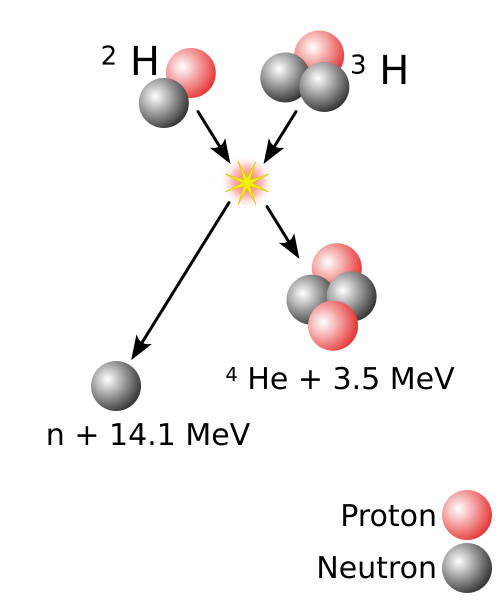
\includegraphics[width=0.7\linewidth]{DuTFusion.png}
            \end{figure}
        \end{column}
        \begin{column}{0,5\linewidth}
            \begin{figure}
                \centering
                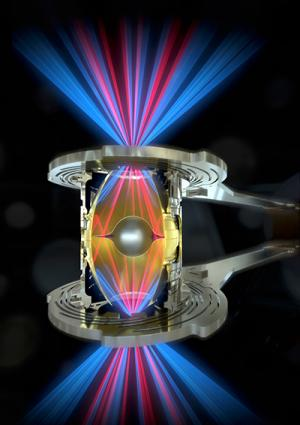
\includegraphics[width=0.7\linewidth]{hohlraum.png}
                % Hohlraum
                \caption*{Hohlraum}
            \end{figure}
        \end{column}
    \end{columns}
    
\end{frame}

\begin{frame}{Inertial Confinement Fusion - Boltzmann Equation}

\vspace{0.2cm}

\begin{center}
\begin{tikzpicture}

% --- Diagram 1: Nuclear Rod Cross-Section ---

\def\h{1.5} % image height
\def\c{6/2} % half image length

% Gold foil outer wall
\filldraw[fill=gray!20, draw=gold, ultra thick] (0,0) rectangle (2*\c,\h);

% Label for gold foil
\node[above] at (\c,\h+0.1) {\small Gold Foil Wall};

% Plastic layer
\filldraw[fill=orange!50, draw=orange!80!black, thick] (\c,\h/2) circle (0.55);
\draw[->, thin] (\c+0.8,\h/2+0.35) -- (\c+0.3,\h/2+0.35);
\node[right] at (\c+0.8,\h/2+0.35) {\tiny Plastic};

% Deuterium layer
\filldraw[fill=cyan!50, draw=cyan!80!black, thick] (\c,\h/2) circle (0.4);
\draw[->, thin] (\c+0.8,\h/2-0.3) -- (\c+0.2,\h/2-0.3);
\node[right] at (\c+0.8,\h/2-0.3) {\tiny Deuterium};

% Core (fuel)
\filldraw[fill=red!70, draw=red!90!black, thick] (\c,\h/2) circle (0.3);
\node at (\c,\h/2) {\tiny Core};

\end{tikzpicture}
\vspace{-0.3cm}
\[
\begin{cases}
    \Omega \cdot \nabla_x \psi + \sigma_t \psi = q+\frac{\sigma_s}{4\pi}\int_{S^2}\psi(x,\Omega)\,d\Omega \\
    \psi:\R^3\times S^2 \to \R \quad x\in\R^3,\Omega\in S^2 \quad \psi(x_{inflow}) = \alpha
\end{cases}
\]
\vspace{-0.3cm}
% Isotropic

% --- Diagram 2: 1D Slab Geometry ---
\begin{tikzpicture}

\def\h{1.5} % image height
\def\c{6/2} % half image length

% Buffer (left)
\filldraw[fill=gray!20, draw=gray, thick] (\c-3,0) rectangle (\c-2,\h);
% Plastic (left)
\filldraw[fill=orange!50, draw=orange!80!black, thick] (\c-2,0) rectangle (\c-1,\h);
% Deuterium (left)
\filldraw[fill=cyan!50, draw=cyan!80!black, thick] (\c-1,0) rectangle (\c-0.5,\h);
% Core
\filldraw[fill=red!70, draw=red!90!black, thick] (\c-0.5,0) rectangle (\c+0.5,\h);
% Deuterium (right)
\filldraw[fill=cyan!50, draw=cyan!80!black, thick] (\c+0.5,0) rectangle (\c+1,\h);
% Plastic (right)
\filldraw[fill=orange!50, draw=orange!80!black, thick] (\c+1,0) rectangle (\c+2,\h);
% Buffer (right)
\filldraw[fill=gray!20, draw=gray, thick] (\c+2,0) rectangle (\c+3,\h);


% Zone labels (below slab)
\node[below, font=\tiny] at (\c-1.5, 0)   {Plastic};
\node[below, font=\tiny] at (\c-0.75, 0)   {D$_2$};
\node[below, font=\tiny] at (\c, 0)   {Core};
\node[below, font=\tiny] at (\c+0.75, 0)   {D$_2$};
\node[below, font=\tiny] at (\c+1.5, 0)   {Plastic};


% Title
\node[above, font=\small] at (\c, \h) {1D Slab Geometry};

% x-axis arrow
%\draw[->] (0, -0.6) -- (\c*2+0.5, -0.6) node[right] {\small $x$};

% Zone boundary ticks
%\foreach \x in {\c-3,\c-2,\c-1,\c-0.5,\c,\c+0.5,\c+1,\c+2,\c+3}{
%    \draw (\x, -0.5) -- (\x, -0.7);
%}

\end{tikzpicture}
\end{center}
\vspace{-0.3cm}
\[
\begin{cases}
    \mu \partial_x \psi + \sigma_t \psi = q+\frac{\sigma_s}{4\pi}\int_{-1}^1\psi(x,\mu)2\pi \,d\mu \\ 
    \psi:\R\times[-1,1] \quad x\in\R,\mu=\Omega\cdot \vec e_1\in[-1,1]\quad \psi(x_{inflow}) = \alpha
    
\end{cases}
\]
\end{frame}

\begin{frame}{Discretized Integral}

    Consider the quadrature of order $\mathcal{L}$: 
    \[\int_{-1}^1\psi(x,\mu)d\mu=\sum_{\ell\in\mathcal{L}}w_\ell \psi(x,\mu_\ell)\]
    Then we have the system of equations:
    \[\mu_\ell\,\partial_x\psi_\ell+\sigma_t \psi_\ell=q+ \frac{\sigma_s}{4\pi } \sum_{\ell \in\mathcal{L}}w_\ell \psi(x,\mu_\ell)\]
    so it makes sense to first solve the simplified equation, an advection-reaction PDE:
    \[\mu_\ell \psi_\ell'(x)+\sigma_t(x) \psi_\ell(x)=q(x) \quad \forall\;\ell \in \mathcal L \]
\end{frame}





\begin{frame}{Setup of Mesh}
We assume that $\sigma_t,\,\sigma_s,\,q(x)$ are constant across zones, and in particular are constant inside a single cell.
\vspace{-5mm}
\begin{center}
\begin{tikzpicture}[x=1.2cm, y=1.2cm, >=stealth]


    % ==========================================
    % VARIABLE DEFINITIONS (Adjust these values)
    % ==========================================
    % Heights
    \pgfmathsetmacro{\Hshade}{2.0}  % Height of the shaded regions
    \pgfmathsetmacro{\Hhat}{1.2}    % Height of the basis functions (chi)
    \pgfmathsetmacro{\Harrow}{2.0}  % Height of the Zone indicator arrows
    \pgfmathsetmacro{\Hdash}{2.5}   % Height of the boundary dashed lines
    \pgfmathsetmacro{\Hlabel}{1.5}  % Vertical position of the zone text 
    
    % Lengths of the different sections
    \pgfmathsetmacro{\LOne}{1.8}    % Length of Zone 1
    \pgfmathsetmacro{\LTwo}{1.8}    % Length of Zone 2
    \pgfmathsetmacro{\LGap}{0.8}    % Length of the dotted gap
    \pgfmathsetmacro{\LMmOne}{1.8}  % Length of Zone M-1
    \pgfmathsetmacro{\LM}{1.8}      % Length of Zone M
    
    % Number of mesh intervals per zone
    \def\NOne{5}
    \def\NTwo{5}
    \def\NMmOne{5}
    \def\NM{6}
    % ==========================================

    % Calculate cumulative x-coordinates of boundaries
    \pgfmathsetmacro{\xO}{0}
    \pgfmathsetmacro{\xA}{\xO + \LOne}
    \pgfmathsetmacro{\xB}{\xA + \LTwo}
    \pgfmathsetmacro{\xC}{\xB + \LGap}
    \pgfmathsetmacro{\xD}{\xC + \LMmOne}
    \pgfmathsetmacro{\xE}{\xD + \LM}

    % Shaded zones (alternating gray/white backgrounds)
    \fill[gray!30] (\xA, 0) rectangle (\xB, \Hshade);
    \fill[gray!30] (\xC, 0) rectangle (\xD, \Hshade);

    % Main x-axis
    \draw[->, thick] (-0.5, 0) -- (\xE + 0.5, 0) node[right] {$x$};

    % Vertical dashed boundaries at the ends of the domain
    \draw[dashed] (\xO, 0) -- (\xO, \Hdash) node[above] {$x = 0$};
    \draw[dashed] (\xE, 0) -- (\xE, \Hdash) node[above] {$x = \ell_D$};

    % Nodes (dots along the axis indicating the mesh)
    \foreach \i in {0,...,\NOne}   \fill (\xO + \i*\LOne/\NOne, 0) circle (1.5pt);
    \foreach \i in {1,...,\NTwo}   \fill (\xA + \i*\LTwo/\NTwo, 0) circle (1.5pt);
    \foreach \i in {0,...,\NMmOne} \fill (\xC + \i*\LMmOne/\NMmOne, 0) circle (1.5pt);
    \foreach \i in {1,...,\NM}     \fill (\xD + \i*\LM/\NM, 0) circle (1.5pt);
    
    % Ellipses for the break/discontinuity in the domain
    \pgfmathsetmacro{\xMidGap}{\xB + \LGap/2}
    \node at (\xMidGap, 0) {$\dots$};
    \node at (\xMidGap, \Hlabel) {$\dots$};
    \node at (\xMidGap, \Harrow) {$\dots$};

    % Zone boundary indicators (double-headed arrows)
    \draw[<->] (\xO, \Harrow) -- (\xA, \Harrow) node[midway, above] {Zone 1};
    \draw[<->] (\xA, \Harrow) -- (\xB, \Harrow) node[midway, above] {Zone 2};
    \draw[<->] (\xC, \Harrow) -- (\xD, \Harrow) node[midway, above] {Zone $M-1$};
    \draw[<->] (\xD, \Harrow) -- (\xE, \Harrow) node[midway, above] {Zone $M$};
    
    % Add crosses at the internal zone boundaries to match the original style
    \node at (\xA, \Harrow) {$\times$};
    \node at (\xD, \Harrow) {$\times$};

    % Zone Properties (sigma and q)
    \node[align=center] at (\xO + \LOne/2, \Hlabel) {$\sigma_{t,1}$ \\[0.5em] $q_1$};
    \node[align=center] at (\xA + \LTwo/2, \Hlabel) {$\sigma_{t,2}$ \\[0.5em] $q_2$};
    \node[align=center] at (\xC + \LMmOne/2, \Hlabel) {$\sigma_{t,M-1}$ \\[0.5em] $q_{M-1}$};
    \node[align=center] at (\xD + \LM/2, \Hlabel) {$\sigma_{t,M}$ \\[0.5em] $q_M$};

    % Basis functions (Linear hat functions)
    
    % Half hat function chi_0 at x=0
    \pgfmathsetmacro{\xHatOneEnd}{\xO + \LOne/\NOne}
    \draw[thick] (\xO, \Hhat) -- (\xHatOneEnd, 0);
    \node[above] at (\xO, \Hhat) {$\chi_0$};
    \node[below=3pt] at (\xO, 0) {$x_0$};

    % Full hat function chi_i at a calculated node inside Zone M-1
    \pgfmathsetmacro{\xHatILeft}{\xC + 2*\LMmOne/\NMmOne}
    \pgfmathsetmacro{\xHatIMid}{\xC + 3*\LMmOne/\NMmOne}
    \pgfmathsetmacro{\xHatIRight}{\xC + 4*\LMmOne/\NMmOne}
    \draw[thick] (\xHatILeft, 0) -- (\xHatIMid, \Hhat) -- (\xHatIRight, 0);
    \node[above] at (\xHatIMid, \Hhat) {$\chi_i$};
    \node[below=3pt] at (\xHatIMid, 0) {$x_i$};

    % Half hat function chi_N at x=ell_D
    \pgfmathsetmacro{\xHatNStart}{\xE - \LM/\NM}
    \draw[thick] (\xHatNStart, 0) -- (\xE, \Hhat);
    \node[above] at (\xE, \Hhat) {$\chi_N$};
    \node[below=3pt] at (\xE, 0) {$x_N$};

\end{tikzpicture}
\end{center}

Standard hat functions $\chi_i \in \mathbb V_h$,  $\chi_i: \R\to[0,1]$, \[\chi_i=\begin{cases}
    \frac{x-x_{i-1}}{x_i-x_{i-1}} & x\in[x_{i-1},x_i] \\
    \frac{x_{i+1}-x}{x_{i+1}-x_i} & x\in[x_i,x_{i+1}] \\
    0 & \text{otherwise}
\end{cases}\]
\end{frame}

\begin{frame}{Finite Elements Formulation (Galerkin)}
    The finite element formulation is:
    
    \begin{multline*}
    \int_{0}^{\ell_D} (\mu \partial_x \psi_h) \chi_i\,dx +  \int_0^{\ell_D}\sigma_t\psi_h\chi_i dx +\underline{\mu \psi_h (x_{\text{in}})  \chi_i(x_{\text{in}})} \\ 
    = \int_{0}^{\ell_D} q\chi_i\,dx + \underline{\mu\alpha \chi_i(x_{\text{in}})}, \quad \forall i = 0, ..., N_h 
    \end{multline*}
    
    The underlined terms are our weakly enforced inflow boundary conditions.
\end{frame}


\begin{frame}{Naive Finite Element Solution}

\begin{columns}[c]

    \begin{column}{0.4\textwidth}
        \begin{figure}
            \centering
            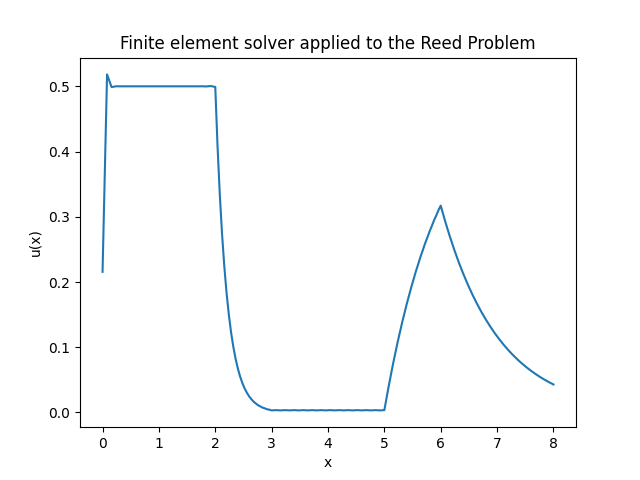
\includegraphics[width=\linewidth]{reed_problem_easy_example.png}
        \end{figure}
        \centering
        \tiny
        \begin{tabular}{c|c|c|c|c|c}
            \hline
            \multicolumn{6}{c}{Reed Problem Benchmark}\\
            \hline
            Length & 2 & 1 & 2 & 1 & 2\\
            Cells & 25 & 25 & 25 & 25 & 25 \\
            $\sigma_t$ & 50 & 5 & 0 & 1 & 1 \\
            $q$ & 25 & 0 & 0 & 0.5 & 0 \\
            \hline
            $\alpha$ & \multicolumn{5}{c}{0.0}  \\
            $\mu$ & \multicolumn{5}{c}{1.0}  \\
            \hline
        \end{tabular}
    \end{column}

    \begin{column}{0.6\textwidth}
        {\small
        \begin{tabular}{ccc}
        \hline
        $h$ & $L^1$ Error & Conv. Rate \\
        \hline
        $4.00 \times 10^{-2}$ & $3.33 \times 10^{-3}$ & --- \\
        $2.00 \times 10^{-2}$ & $8.72 \times 10^{-4}$ & $1.93$ \\
        $1.00 \times 10^{-2}$ & $2.21 \times 10^{-4}$ & $1.98$ \\
        $5.00 \times 10^{-3}$ & $5.54 \times 10^{-5}$ & $2.00$ \\
        $2.50 \times 10^{-3}$ & $1.39 \times 10^{-5}$ & $2.00$ \\
        $1.25 \times 10^{-3}$ & $3.47 \times 10^{-6}$ & $2.00$ \\
        $6.25 \times 10^{-4}$ & $8.67 \times 10^{-7}$ & $2.00$ \\
        $3.13 \times 10^{-4}$ & $2.17 \times 10^{-7}$ & $2.00$ \\
        \hline
        \end{tabular}
        }
    \end{column}

\end{columns}

\end{frame}

\begin{frame}{What Goes Wrong?}

    Although the numerical method is convergent in $||\cdot||_{L^1}$, the gradient was not bounded and thus there is no control on the oscillations of the solution.

    Internal boundary layers appear when $\sigma_t$ changes rapidly; this leads to instability.
    
    \begin{columns}[cc]

        \begin{column}{0.5\textwidth}
            \begin{figure}
                \centering
                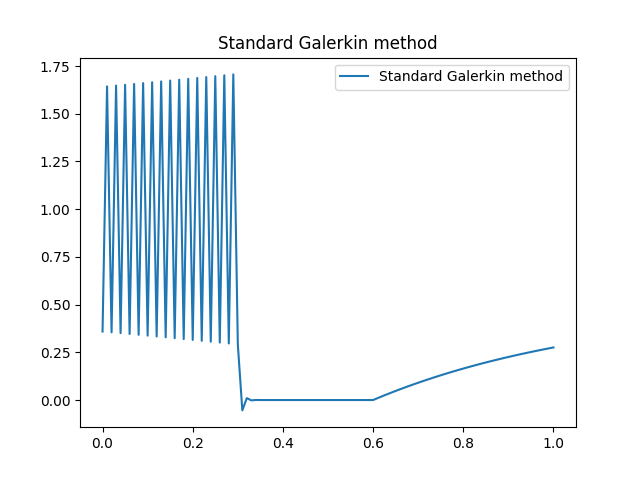
\includegraphics[width=\linewidth]{galerkin_instability.png}
            \end{figure}
       \end{column}

    \begin{column}{0.5\textwidth}
       \small
        \begin{tabular}{c|c|c|c}
            \hline
            \multicolumn{4}{c}{Boundary Value Benchmark}\\
            \hline
            Length & 0.3 & 0.3 & 0.4\\
            Cells & 30 & 30 & 40\\
            $\sigma_t$ & 1.0 & $1 \times 10^{5}$ & 2\\
            $q$ & 1.0 & 0.0 & 1.0\\
            \hline
            $\alpha$ & \multicolumn{3}{c}{1.0}  \\
            $\mu$ & \multicolumn{3}{c}{1.0}  \\
            \hline
        \end{tabular}

    \end{column}


\end{columns}

\end{frame}


\begin{frame}{Streamline Upwind Petrov–Galerkin (SUPG)} %'sup G%

The Petrov method involves continuing to use $\mathbb V_h$ as the trial space where the solution lives, but now the test functions are in: 
\[
\mathbb W_h : = \operatorname{span}_{i \in \text{Vertices}} \lt\{\chi_i (x) + \sum_{K \in \text{Cells}} \tau_K \mu \, \chi'_{|K}(x)\rt\}, \;  \tau_K = \frac{h_K}{2|\mu|} \frac{1}{\max(1, \sigma_th_K)}
\]
Note $\tau_K = 0$ is Galerkin.

\begin{center}
\begin{tikzpicture}[xscale=1, yscale=1]

    % Axis line
    \draw[thick] (-4.5, 0) -- (4.5, 0);

    % Dots at the ends of the axis
    \node at (-4.8, 0) {$\dots$};
    \node at (4.8, 0) {$\dots$};

    % Axis nodes (dots)
    \foreach \x in {-4, -2, 0, 2, 4} {
        \fill (\x, 0) circle (1.2pt);
    }

    % Label for x_i
    \node[below] at (0, -0.1) {$x_i$};

    % Standard hat function (dashed)
    \draw[thick, dashed] (-2, 0) -- (0, 2) -- (2, 0);

    % Label for chi_i
    \node[right] at (0.1, 1.9) {$\chi_i$};

    % SUPG test function (solid, thick)
    % The slopes are kept parallel to the dashed hat function (slope = 1 and -1)
    % Left segment (shifted up)
    \draw[line width=1.5pt] (-2, 0.8) -- (0, 2.8);
    % Right segment (shifted down)
    \draw[line width=1.5pt] (0, 1.2) -- (2, -0.8);

    % Label for eta(chi_i)
    \node[left] at (-0.5, 2.5) {$\eta(\chi_i) \in \mathbb{W}_h$};

    % Vertical dotted lines connecting to nodes
    \draw[dotted, thick] (-2, 0) -- (-2, 0.8);
    \draw[dotted, thick] (0, 0) -- (0, 2.8);
    \draw[dotted, thick] (2, -0.8) -- (2, 0);
\end{tikzpicture}
\end{center}
\end{frame}

\begin{frame}{SUPG Results}

For the previous problem with boundary layers, SUPG performs much better.
\begin{columns}[cc]

    \begin{column}{0.5\textwidth}
        \centering
        \begin{figure}
            \centering
            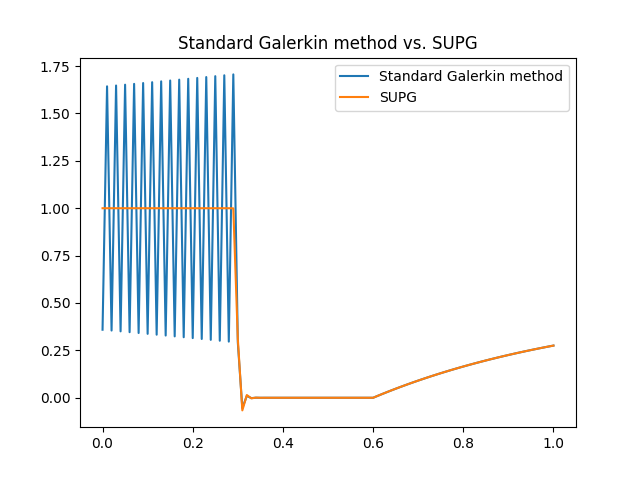
\includegraphics[width=\linewidth]{galerkin_vs_supg.png}

        \end{figure}
    \end{column}
    
    \begin{column}{0.5\textwidth}
        \centering
       \small
        \begin{tabular}{c|c|c|c}
            \hline
            \multicolumn{4}{c}{Boundary Value Benchmark}\\
            \hline
            Length & 0.3 & 0.3 & 0.4\\
            Cells & 30 & 30 & 40\\
            $\sigma_t$ & 1.0 & $1 \times 10^{5}$ & 2\\
            $q$ & 1.0 & 0.0 & 1.0\\
            \hline
            $\alpha$ & \multicolumn{3}{c}{1.0}  \\
            $\mu$ & \multicolumn{3}{c}{1.0}  \\
            \hline
        \end{tabular}
    \end{column}

\end{columns}



\end{frame}

\begin{frame}{SUPG Results}
    This method is stable around boundary layers (large changes in $\sigma_t$), but with a coarse mesh it does not converge quadratically around them.
    \begin{figure}
        \centering
        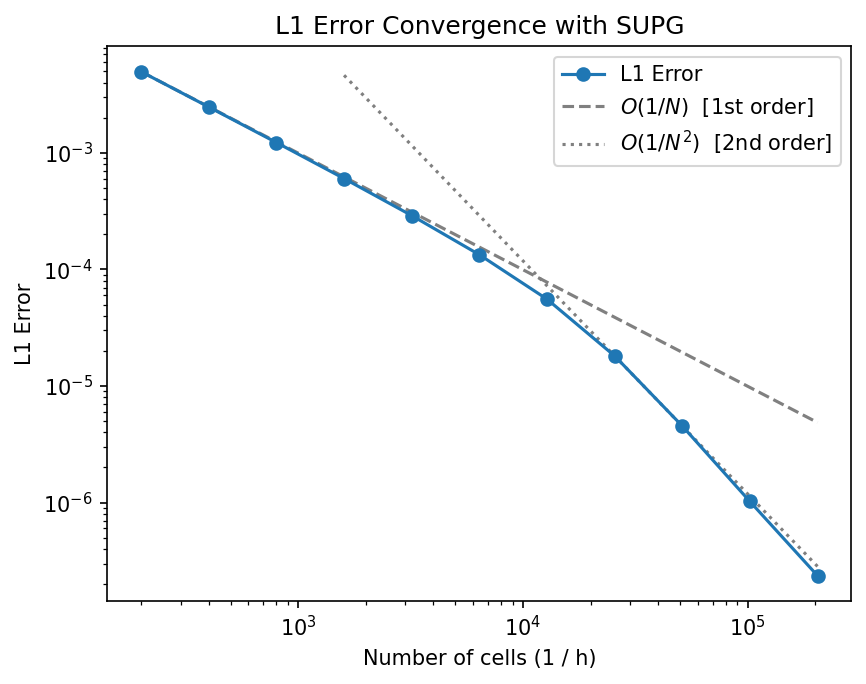
\includegraphics[width=0.6\linewidth]{convergence_plot.png}
    \end{figure}
\end{frame}


\begin{frame}{Reintroducing Integral Term}

    Now that we can solve each individual Advection-Reaction Equation:
    \[\mu_\ell \psi_\ell'(x)+\sigma_t(x)\psi_\ell(x)=q(x) \quad \forall\;\ell \in\mathcal{L}\]
    We can return to the system of equations:
    
    \[\mu_\ell\,\partial_x\psi_\ell+\sigma_t \psi_\ell=q+ \frac{\sigma_s}{4\pi } \sum_{\ell \in\mathcal{L}}w_\ell \psi(x,\mu_\ell)\]
    Thus, the system we want to solve is a system of differential equations (for each $\ell \in \mathcal L$) coupled by the RHS.
    
\end{frame}


\begin{frame}{Richardson Iteration}

When we discretize our mesh and use the finite element method to solve the differential equations, we get a very large linear system.  

    \begin{center}
        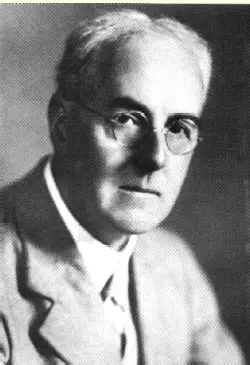
\includegraphics[scale= 0.35]{richard.png}
    \end{center}

Solving it is impractical, but because the only coupling term is the flux integral, we can use Richardson iteration.

\end{frame}
\begin{frame}{Richardson Iteration (cont.)}

\hline
\textbf{Algorithm:} Richardson Iteration for Transport
\hline
    \begin{enumerate}
        \item Take a scalar flux guess $\phi^{(0)} =  0$
        
        \item Solve the system of differential equations using our scalar flux guess. $\mu_\ell \frac{d\psi^{\ell,(k)}}{dx} + \sigma_t(x) \psi^{\ell,(k)}(x) = q(x) + \frac{\sigma_s(x)}{4\pi} \phi^{(k)}(x)$
        
        \item Calculate a new scalar flux guess using quadrature with our solutions to the system of equations. $\phi^{(k+1)}(x) = \sum_{\ell' \in \mathcal{L}} w_{\ell'} \psi^{\ell',(k)}(x)$

        \item Repeat until convergence.
    \end{enumerate}
For problems where $\frac{\sigma_t - \sigma_s}{\sigma_t} \approx O(1)$, i.e. sufficiently high absorption, Banach fixed point theorem guarantees convergence, so the algorithm works.
\end{frame}

\begin{frame}{Reed Problem Across All Angles}

    \begin{columns}[cc]
    
        \begin{column}{0.5\textwidth}
            \begin{figure}
                \centering
                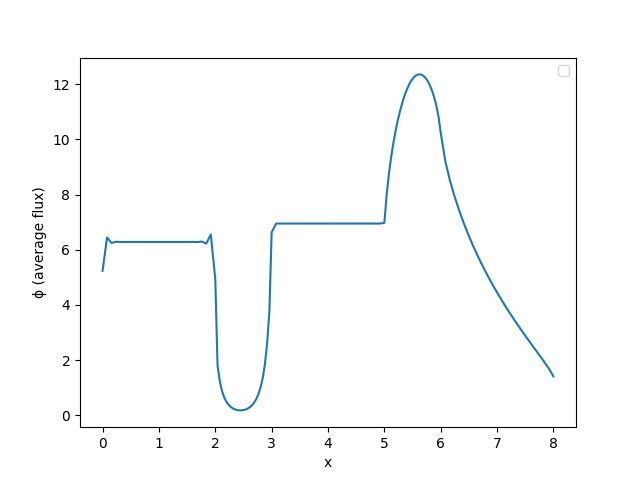
\includegraphics[width=\linewidth]{reed_problem_phi.png}
            \end{figure}
            
            \tiny
            \centering
            \begin{tabular}{c|c|c|c|c|c}
                \hline
                \multicolumn{6}{c}{Reed Problem Benchmark}\\
                \hline
                Length & 2 & 1 & 2 & 1 & 2\\
                Cells & 25 & 25 & 25 & 25 & 25 \\
                $\sigma_t$ & 50 & 5 & 0 & 1 & 1 \\
                $\sigma_s$ & 0& 0& 0 & 0.9 & 0.9 \\ 
                $q$ & 25 & 0 & 0 & 0.5 & 0 \\
                \hline
                $\alpha$ & \multicolumn{5}{c}{0.0}  \\
                Angles & \multicolumn{5}{c}{32}  \\
                \hline
            \end{tabular}
        \end{column}
    
        \begin{column}{0.5\textwidth}
            \begin{figure}
                \centering
                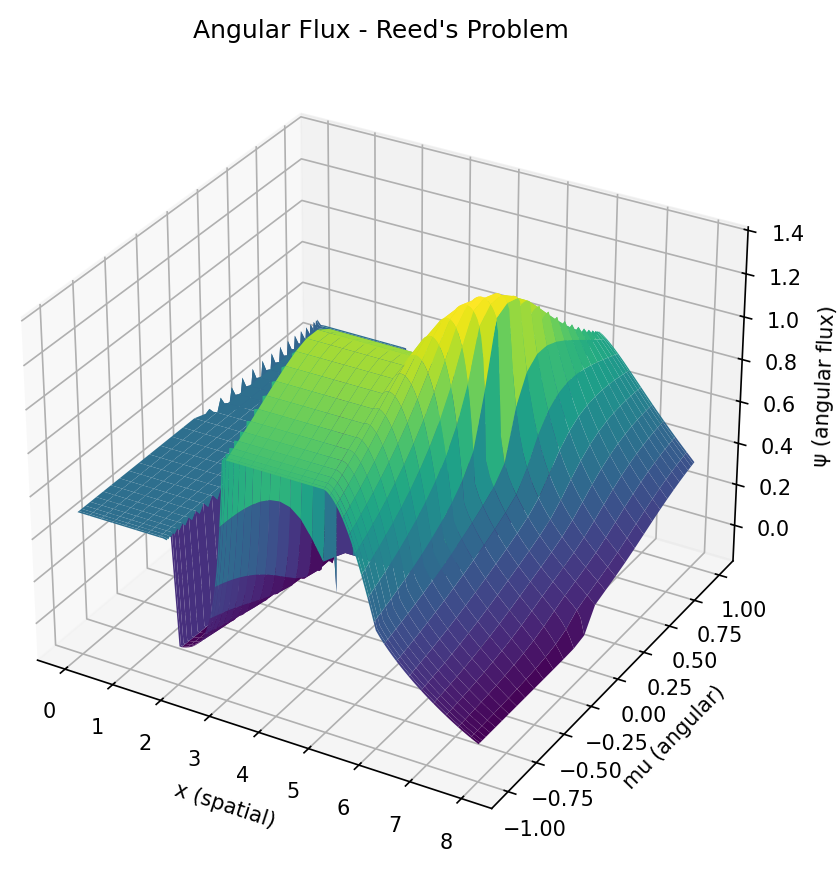
\includegraphics[width=\linewidth]{reed_problem_3d.png}
            \end{figure}
        \end{column}
    
    \end{columns}
\end{frame}

\begin{frame}{Preconditioning}

In the regime where $\sigma_s >> \sigma_a$, Richardson iteration needs exponentially more steps to converge, which quickly becomes prohibitive.

\hspace{}

\begin{columns}[onlytextwidth]
    \begin{column}{0.5\textwidth}
        \centering
        \begin{tabular}{c|c}
        \hline
            \multicolumn{1}{c}{$\sigma_s/ \sigma_t$} & \multicolumn{1}{c}{Iterations} 
            \\ \hline
            0.0 & 1\\
            0.25 & 14\\
            0.5 & 27\\
            0.9 & 174\\
            1.0 & 57006\\
            \hline
        \end{tabular}
    \end{column}
    \begin{column}{0.5\textwidth}
        \centering
        \small 
        \begin{tabular}{c|c}
            \hline
            \multicolumn{2}{c}{Scattering Benchmark}\\
            \hline
            Length & 10\\
            Cells & 100 \\
            $\sigma_t$ & 10 \\
            $q$ & 0.05 \\
            \hline
            $\alpha$ & \multicolumn{1}{c}{1.0}  \\
            Angles & \multicolumn{1}{c}{8}  \\
            \hline
        \end{tabular}

    \end{column}
\end{columns}
\end{frame}

\begin{frame}{Preconditioning (cont.)}

We assume $\sigma_s \sim 1/\eps$, $\sigma_a \sim \eps$. Via the method of asymptotic expansion, we introduce 
\[
\psi = \psi^{(0)} + \eps \psi^{(1)} + \eps^2 \psi^{(2)} + \cdots \text{ as } \eps \to 0
\] into \[
\Omega \cdot \nabla_x \psi^\eps(x, \Omega) + \frac{\sigma_t}{\eps} \psi^\eps (x, \Omega) = \eps q(x) + \frac{1}{4\pi} \lt[ \frac{\sigma_t}{\eps} - \sigma_a \eps \rt] \int_{S^2} \psi^\eps(x, \Omega') d\Omega'
\] 
By grouping the $o(1/\eps), \, o(1), \, o(\eps), ...$ terms we see that the former dominates, and we obtain a Poisson PDE: \[
-\nabla \cdot \lt( \frac{1}{3\sigma_t} \nabla \psi^{(0)}(x) \rt) + \sigma_a \psi^{(0)}(x) = 4\pi q(x) 
\]
\end{frame}

\begin{frame}{Preconditioning (cont.)}

Define a mapping $r \mapsto \Phi_h(r)$.

Multiplying by a test function $v_h \in \mathbb{V}_h$ and using integration by parts gives:

 \begin{multline*}
    \int_0^{\ell_D} \frac{1}{3\sigma_t} \Phi_h(r)' v_h' dx + \int_0^{\ell_D} \sigma_a \Phi_h(r) v_h dx \\
    + \frac{\overline \omega}{4} \lt\{\Phi_h(r) (0) v_h(0) + \Phi_h(r)(\ell_D) v_h(\ell_D)\rt\} = \int_0^{\ell_D} r\, dx 
 \end{multline*}   

 We can solve this via classical Finite Element Method.
  
    
\end{frame}

\begin{frame}{Preconditioning (cont.)}

Let $\Phi_h$ be the FEM solution operator for our Poisson problem.

We use $M := \mathbb{I} + \Phi_h$ as a preconditioner for our Richardson iteration!

\hspace{}

\begin{columns}[onlytextwidth]
    \begin{column}{0.5\textwidth}
        \centering
        \begin{tabular}{c|c}
        \hline
            \multicolumn{1}{c}{$\sigma_s/ \sigma_t$} & \multicolumn{1}{c}{Iterations} 
            \\ \hline
            0.0 & 1\\
            0.25 & 5\\
            0.5 & 6\\
            0.9 & 10\\
            1.0 & 22\\
            \hline
        \end{tabular}
    \end{column}
    \begin{column}{0.5\textwidth}
        \centering
        \small 
        \begin{tabular}{c|c}
            \hline
            \multicolumn{2}{c}{Scattering Benchmark}\\
            \hline
            Length & 10\\
            Cells & 100 \\
            $\sigma_t$ & 10 \\
            $q$ & 0.05 \\
            \hline
            $\alpha$ & \multicolumn{1}{c}{1.0}  \\
            Angles & \multicolumn{1}{c}{8}  \\
            \hline
        \end{tabular}

    \end{column}
\end{columns}

\end{frame}

\begin{frame}{Grazing Problem}
    Consider boundary condition imposed on the "grazing" direction:
    \[\psi(0,\mu)=\begin{cases}
        1 & \mu=\mu_0\approx 0 \\
        0 & \text{else}
    \end{cases}\]

\begin{columns}[cc]
    \begin{column}{0.5\textwidth}
        \centering
        \begin{figure}
        \centering
        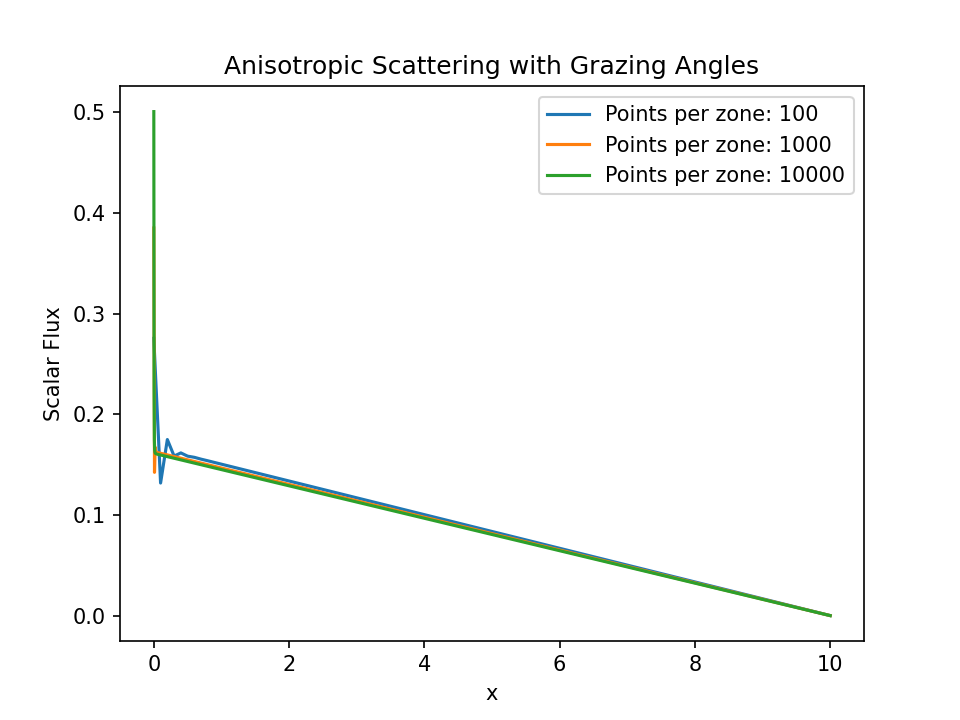
\includegraphics[width=\linewidth]{grazing.png}
    \end{figure}
    \end{column}
    \begin{column}{0.5\textwidth}
        \centering
        \small 
        \begin{tabular}{c|c}
            \hline
            \multicolumn{2}{c}{Grazing Benchmark}\\
            \hline
            Length & 10\\
            Cells & 100 \\
            $\sigma_t$ & 100 \\
            $\sigma_s$ & 100 \\
            $q$ & 0.0 \\
            \hline
            $\psi_0(\mu)$ & \multicolumn{1}{c}{1.0}  \\
            Angles & \multicolumn{1}{c}{8}
        \end{tabular}

    \end{column}
\end{columns}
    
\end{frame}

\begin{frame}{Internal Boundary Layer - Grazing Problem}
    \begin{figure}
        \centering
        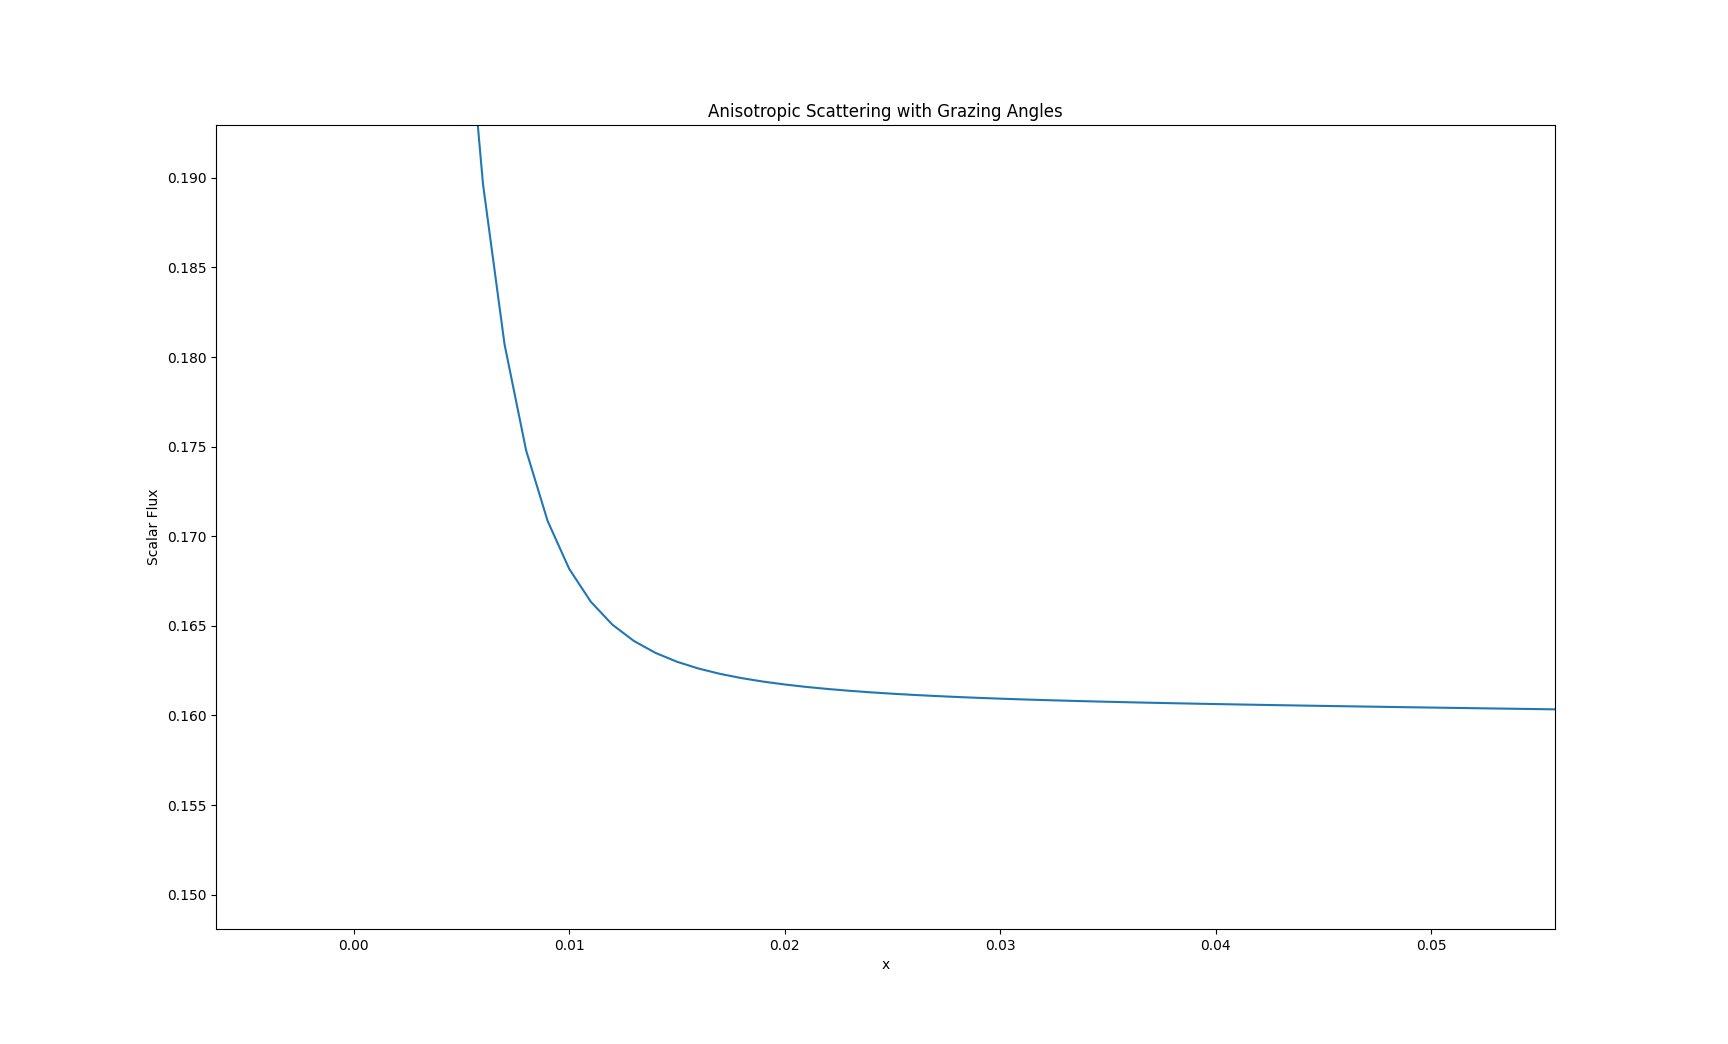
\includegraphics[width=1\linewidth]{grazing_ibl.png}
    \end{figure}
\end{frame}

\begin{frame}{Takeaways}
    \begin{itemize}
        \item Moving from theory to implementation takes tremendous care
        \item Good coding practices and test cases are vital
        \item Organizing code is essential as the project scales
        \item Rigorous justification of our methods is harder than writing them
    \end{itemize}
\end{frame}

\begin{frame}{Conclusion}
\begin{enumerate}
    \item Radiation Transport Equation
    \item Naive Method for Advection-Reaction via Galerkin
    \item Improved Method via SUPG
    \item Reintroduced Integral Term 
    \item Richardson Iteration
    \item Preconditioning
\end{enumerate}
\end{frame}

\begin{frame}{Acknowledgments}
    \begin{columns}[cc]
        \begin{column}{0.5\linewidth}
            \begin{figure}
                \centering
                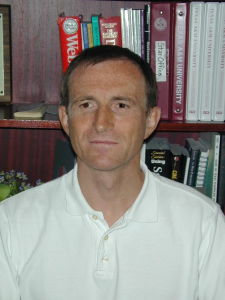
\includegraphics[width=0.7\linewidth]{guermond.png}
            \caption*{Prof. Guermond}
            \end{figure}
        \end{column}
        \begin{column}{0,5\linewidth}
            \begin{figure}
                \centering
                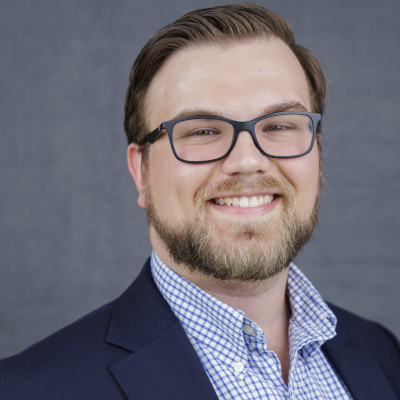
\includegraphics[width=0.7\linewidth]{image.png}
                \caption*{Jordan Hoffart}
            \end{figure}
        \end{column}
    \end{columns}
\end{frame}


\begin{frame}{Appendix A: a priori 1-D energy estimate}
\[\mu u'(x) + \sigma_t(x)u(x) = q(x), \quad u(x_\text{inflow})=\alpha\]
\[\mu u' + \sigma_t u+ \frac{1}{2}(|\mu\vec e_1 \cdot \vec n|-\mu\vec e_1 \cdot \vec n)u = q +\frac{1}{2}(|\mu\vec e_1 \cdot \vec n|-\mu\vec e_1 \cdot \vec n)\alpha\]
\[v\lt[\mu u' + \sigma_t u+ \frac{1}{2}(|\mu\vec e_1 \cdot \vec n|-\mu\vec e_1 \cdot \vec n)u \rt] = v \lt[q +\frac{1}{2}(|\mu\vec e_1 \cdot \vec n|-\mu\vec e_1 \cdot \vec n)\alpha\rt]\]
\[
\int_D \mu v u' dx + \int_D \sigma_t vu \,  dx +\frac{1}{2}\int_{\partial D}(|\mu\vec e_1 \cdot \vec n|-\mu\vec e_1 \cdot \vec n)uv \, dx\]
 \[= \int_D vq+\frac{1}{2}\int_{\partial D}(|\mu\vec e_1 \cdot \vec n|-\mu\vec e_1 \cdot \vec n)\alpha \, dx, \quad \,  \forall\, v\in\mathbb{V}_h.\]

\end{frame}

\begin{frame}{Appendix A (cont.)}
Now let $v = u$ for the energy estimate and we have  
\[\int_D \mu u u' dx + \int_D \sigma_t uu dx +\frac{1}{2}\int_{\partial D}(|\mu\vec e_1 \cdot \vec n|-\mu\vec e_1 \cdot \vec n)u^2\, dx\]  
\[=\int_D uq+\frac{1}{2}\int_{\partial D}(|\mu\vec e_1 \cdot \vec n|-\mu\vec e_1 \cdot \vec n)\alpha u \, dx\]
\[\frac{\mu}{2}\int_D (u^2)'   dx +  \sigma_t\int_D u^2 dx = \int_D u(x)q(x) \leq ||u||_2 ||q||_2 \leq \frac{||u||_2^2}{2\eps} + \frac{\eps||q||_2^2}{2}\]
\[
\frac{\mu }{2}\lt.u^2\rt|_{\partial D}+ \sigma_t||u||_2^2  \leq \frac{\sigma_t||u||_2^2}{2} + \frac{||q||_2^2}{2\sigma_{t}} + \frac{1}{2}\int_{\partial D}(|\mu\vec e_1 \cdot \vec n|-\mu\vec e_1 \cdot \vec n)\alpha u \, dx 
\]
\[
\frac{\mu }{2}\lt.u^2\rt|_{\partial D}+ \frac{\sigma_t}{2}||u||_2^2  \leq  \frac{||q||_2^2}{2\sigma_{t}} + \frac{1}{2}\int_{\partial D}(|\mu\vec e_1 \cdot \vec n|-\mu\vec e_1 \cdot \vec n)\alpha u \, dx 
\]
\[\min  \sigma_t ||u||_2^2 \leq \frac{||q||_2^2}{ \min \sigma_t}+  |\mu\vec e_1\cdot \vec n|\alpha^2\]
\end{frame}

\begin{frame}{Appendix B: Energy estimate in $\R^n$}
We begin with the following advection-reaction equation with boundary condition: 
\[
\Omega \cdot \nabla_x u + \sigma_t u = q, \quad u(x_{inflow}) = \alpha
\]
We ``weakly'' incorporate the inflow condition into the PDE:
\begin{align*}
   \int_D u(\Omega \cdot \nabla_x u)+ \int_D \sigma_t u^2 + \int_{\partial D} \frac{1}{2}(|\Omega \cdot \vec n|- \Omega \cdot \vec n) u^2 \\
   = \int_D qu + \frac{1}{2}\int_{\partial D}(|\Omega \cdot \vec n|-  \Omega \cdot \vec n)\alpha  u
\end{align*}
\[
\int_D u(\Omega \cdot \nabla_x u) = \int_D \Omega \cdot u \nabla_x u =  \frac{1}{2}\int_D  \nabla_x\cdot (u^2\Omega) = \frac{1}{2} \int_{\partial D} u^2 \Omega \cdot \vec n \, dS
\]
\end{frame}

\begin{frame}{Appendix B (cont.)}
\begin{align*}
 \int_D \sigma_t u^2 - \int_{\partial D^-} u^2 \Omega \cdot \vec n + \frac{1}{2} \int_{\partial D} u^2 \Omega \cdot \vec n \\
 = \int_D \sigma_tu^2 - \frac{1}{2}\int_{\partial D^-} u^2 \Omega \cdot \vec n + \frac{1}{2}\int_{\partial D^+} u^2 \Omega \cdot \vec n \\
 =  \int_D qu -  \int_{\partial D^-} (\Omega \cdot \vec n )\alpha u \\
 \leq \frac{||q||_2^2}{2\min \sigma_t} + \frac{\min \sigma_t||u||_2^2}{2} - \int_{\partial D^-} (\Omega \cdot \vec n) \alpha u
\end{align*}
\begin{align*}
    \frac{1}{2}\min \sigma_t ||u||_2^2 - \frac{1}{2} \int_{\partial D^{-}}  u^2\Omega \cdot \vec n + \frac{1}{2}\int_{\partial D^+} u^2\Omega \cdot \vec n \\
    \leq \frac{||q||^2_2}{2 \min \sigma_t}   - \int_{\partial D^-} (\Omega \cdot \vec n) \alpha u
\end{align*}


\end{frame}

\begin{frame}{Appendix B (cont.)}
\[\int_{\partial D^-} |\alpha u| \leq ||u||_2||\alpha||_2 \leq \frac{||u||_2^2}{2} + \frac{||\alpha||_2^2}{2}\]\[ \int_{\partial D^-}  |(\Omega \cdot \vec n)\alpha u| \leq -\frac{1}{2}\int_{\partial D^-} (\Omega \cdot \vec n)u^2 -\frac{1}{2} \int_{\partial D^-} (\Omega \cdot \vec n) \alpha ^2 \]
So consider \[
\frac{1}{2}\min \sigma_t ||u||_2^2 - \frac{1}{2} \int_{\partial D^{-}}  u^2\Omega \cdot \vec n + \frac{1}{2}\int_{\partial D^+} u^2\Omega \cdot \vec n
\]
once more and notice that we can cancel the leftmost term of the RHS above, also the the other boundary condition on the LHS is strictly positive, and so we have as before \[
 \min  \sigma_t ||u||_2^2 \leq \frac{||q||_2^2}{ \min \sigma_t} - \int_{\partial D^-} (\Omega \cdot \vec n)\alpha^2 
\]
\end{frame}




\begin{frame}{Appendix C: Better 1-D Bound and Existence}
    \[
    I(x)u' + (\sigma_t/\mu) I(x) u = q/\mu I(x) \Longleftrightarrow (I(x)u)' = (q/\mu)I(x)
    \]
    since $I'(x) = \frac{\sigma_t(x)}{\mu}I(x)$. Then, \[
 u(x) = \frac{1}{\mu I(x)} \int_0^x q I(s) ds
\]
\[
= \frac{1}{\mu} \exp\lt(-\frac{1}{\mu} \int_0^x \sigma_t(\tau) d\tau \rt) \int_0^x q \exp\lt(\frac{1}{\mu} \int_0^s \sigma_t(\tau) d\tau\rt) d s
\]
\end{frame}
\begin{frame}{Appendix C (cont.)}
\[
= \frac{1}{\mu}  \int_0^x q \exp\lt(-\frac{1}{\mu} \int_0^x \sigma_t(\tau) d\tau \rt)\exp\lt(\frac{1}{\mu} \int_0^s \sigma_t(\tau) d\tau\rt) d s
\]
\[
= \frac{1}{\mu}  \int_0^x q \exp\lt(-\frac{1}{\mu} \int_s^x \sigma_t(\tau) d\tau\rt) d s
\]
By assumption $\sigma_t > 0 $, so $\exp(\cdots) \leq 1$ and \[ |u(x)| \leq \frac{1}{\mu} \int_0^x q  \, ds  \leq \frac{1}{\mu} ||q||_2 \sqrt x \]
\[
||u||_2^2 = \int_0^L |u|^2 \, dx \leq \int_0^L \frac{1}{\mu^2} ||q||_2^2 x\, dx \leq \frac{||q||_2^2}{\mu^2}L\]
\[
||u||_2 \leq \frac{||q||_2}{\mu} \sqrt{L}
\]
\end{frame}

\begin{frame}{Appendix D: Uniqueness}
 We could use either estimate to show this, but the second is more obvious. Suppose that $u_1$ and $u_2$ both satisfy \[
 \mu u'(x) + \sigma_t(x) u(x) = q(x), \quad u(x_{\text{inflow}} ) = \alpha
 \]
 then $u_1 -u_2 = v$ satisfies \[
 \mu v'(x) + \sigma_t(x) v(x) = 0, \quad v(x_{\text{inflow}}) = 0 
 \]
 and
 \[
 ||v||_2^2 = \int v^2 \leq 0 \implies v = u_1 - u_2 = 0
 \]
\end{frame}


\end{document}
